\documentclass[1p]{elsarticle_modified}
%\bibliographystyle{elsarticle-num}

%\usepackage[colorlinks]{hyperref}
%\usepackage{abbrmath_seonhwa} %\Abb, \Ascr, \Acal ,\Abf, \Afrak
\usepackage{amsfonts}
\usepackage{amssymb}
\usepackage{amsmath}
\usepackage{amsthm}
\usepackage{scalefnt}
\usepackage{amsbsy}
\usepackage{kotex}
\usepackage{caption}
\usepackage{subfig}
\usepackage{color}
\usepackage{graphicx}
\usepackage{xcolor} %% white, black, red, green, blue, cyan, magenta, yellow
\usepackage{float}
\usepackage{setspace}
\usepackage{hyperref}

\usepackage{tikz}
\usetikzlibrary{arrows}

\usepackage{multirow}
\usepackage{array} % fixed length table
\usepackage{hhline}

%%%%%%%%%%%%%%%%%%%%%
\makeatletter
\renewcommand*\env@matrix[1][\arraystretch]{%
	\edef\arraystretch{#1}%
	\hskip -\arraycolsep
	\let\@ifnextchar\new@ifnextchar
	\array{*\c@MaxMatrixCols c}}
\makeatother %https://tex.stackexchange.com/questions/14071/how-can-i-increase-the-line-spacing-in-a-matrix
%%%%%%%%%%%%%%%

\usepackage[normalem]{ulem}

\newcommand{\msout}[1]{\ifmmode\text{\sout{\ensuremath{#1}}}\else\sout{#1}\fi}
%SOURCE: \msout is \stkout macro in https://tex.stackexchange.com/questions/20609/strikeout-in-math-mode

\newcommand{\cancel}[1]{
	\ifmmode
	{\color{red}\msout{#1}}
	\else
	{\color{red}\sout{#1}}
	\fi
}

\newcommand{\add}[1]{
	{\color{blue}\uwave{#1}}
}

\newcommand{\replace}[2]{
	\ifmmode
	{\color{red}\msout{#1}}{\color{blue}\uwave{#2}}
	\else
	{\color{red}\sout{#1}}{\color{blue}\uwave{#2}}
	\fi
}

\newcommand{\Sol}{\mathcal{S}} %segment
\newcommand{\D}{D} %diagram
\newcommand{\A}{\mathcal{A}} %arc


%%%%%%%%%%%%%%%%%%%%%%%%%%%%%5 test

\def\sl{\operatorname{\textup{SL}}(2,\Cbb)}
\def\psl{\operatorname{\textup{PSL}}(2,\Cbb)}
\def\quan{\mkern 1mu \triangleright \mkern 1mu}

\theoremstyle{definition}
\newtheorem{thm}{Theorem}[section]
\newtheorem{prop}[thm]{Proposition}
\newtheorem{lem}[thm]{Lemma}
\newtheorem{ques}[thm]{Question}
\newtheorem{cor}[thm]{Corollary}
\newtheorem{defn}[thm]{Definition}
\newtheorem{exam}[thm]{Example}
\newtheorem{rmk}[thm]{Remark}
\newtheorem{alg}[thm]{Algorithm}

\newcommand{\I}{\sqrt{-1}}
\begin{document}

%\begin{frontmatter}
%
%\title{Boundary parabolic representations of knots up to 8 crossings}
%
%%% Group authors per affiliation:
%\author{Yunhi Cho} 
%\address{Department of Mathematics, University of Seoul, Seoul, Korea}
%\ead{yhcho@uos.ac.kr}
%
%
%\author{Seonhwa Kim} %\fnref{s_kim}}
%\address{Center for Geometry and Physics, Institute for Basic Science, Pohang, 37673, Korea}
%\ead{ryeona17@ibs.re.kr}
%
%\author{Hyuk Kim}
%\address{Department of Mathematical Sciences, Seoul National University, Seoul 08826, Korea}
%\ead{hyukkim@snu.ac.kr}
%
%\author{Seokbeom Yoon}
%\address{Department of Mathematical Sciences, Seoul National University, Seoul, 08826,  Korea}
%\ead{sbyoon15@snu.ac.kr}
%
%\begin{abstract}
%We find all boundary parabolic representation of knots up to 8 crossings.
%
%\end{abstract}
%\begin{keyword}
%    \MSC[2010] 57M25 
%\end{keyword}
%
%\end{frontmatter}

%\linenumbers
%\tableofcontents
%
\newcommand\colored[1]{\textcolor{white}{\rule[-0.35ex]{0.8em}{1.4ex}}\kern-0.8em\color{red} #1}%
%\newcommand\colored[1]{\textcolor{white}{ #1}\kern-2.17ex	\textcolor{white}{ #1}\kern-1.81ex	\textcolor{white}{ #1}\kern-2.15ex\color{red}#1	}

{\Large $\underline{12a_{0320}~(K12a_{0320})}$}

\setlength{\tabcolsep}{10pt}
\renewcommand{\arraystretch}{1.6}
\vspace{1cm}\begin{tabular}{m{100pt}>{\centering\arraybackslash}m{274pt}}
\multirow{5}{120pt}{
	\centering
	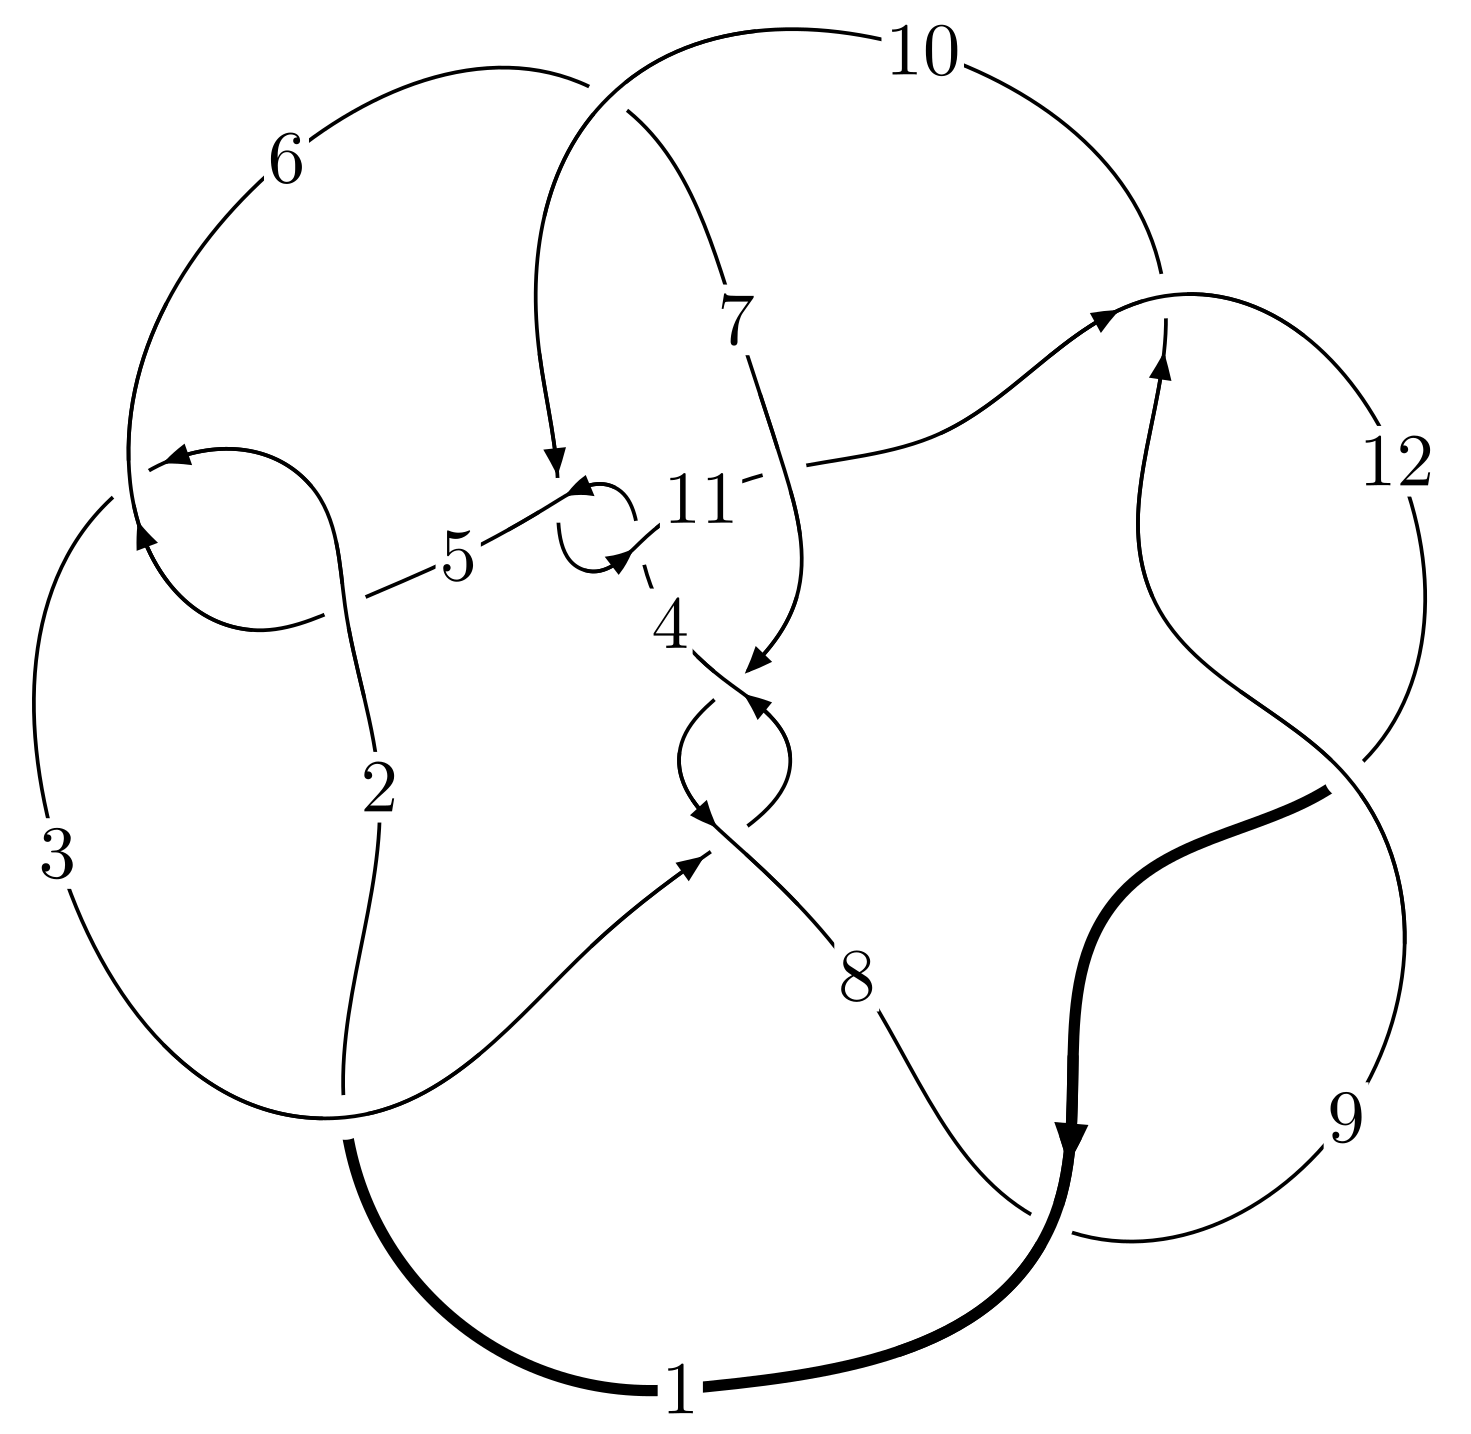
\includegraphics[width=112pt]{../../../GIT/diagram.site/Diagrams/png/1121_12a_0320.png}\\
\ \ \ A knot diagram\footnotemark}&
\allowdisplaybreaks
\textbf{Linearized knot diagam} \\
\cline{2-2}
 &
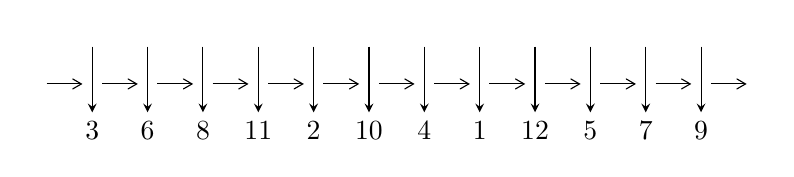
\begin{tikzpicture}[x=20pt, y=17pt]
	% nodes
	\node (C0) at (0, 0) {};
	\node (C1) at (1, 0) {};
	\node (C1U) at (1, +1) {};
	\node (C1D) at (1, -1) {3};

	\node (C2) at (2, 0) {};
	\node (C2U) at (2, +1) {};
	\node (C2D) at (2, -1) {6};

	\node (C3) at (3, 0) {};
	\node (C3U) at (3, +1) {};
	\node (C3D) at (3, -1) {8};

	\node (C4) at (4, 0) {};
	\node (C4U) at (4, +1) {};
	\node (C4D) at (4, -1) {11};

	\node (C5) at (5, 0) {};
	\node (C5U) at (5, +1) {};
	\node (C5D) at (5, -1) {2};

	\node (C6) at (6, 0) {};
	\node (C6U) at (6, +1) {};
	\node (C6D) at (6, -1) {10};

	\node (C7) at (7, 0) {};
	\node (C7U) at (7, +1) {};
	\node (C7D) at (7, -1) {4};

	\node (C8) at (8, 0) {};
	\node (C8U) at (8, +1) {};
	\node (C8D) at (8, -1) {1};

	\node (C9) at (9, 0) {};
	\node (C9U) at (9, +1) {};
	\node (C9D) at (9, -1) {12};

	\node (C10) at (10, 0) {};
	\node (C10U) at (10, +1) {};
	\node (C10D) at (10, -1) {5};

	\node (C11) at (11, 0) {};
	\node (C11U) at (11, +1) {};
	\node (C11D) at (11, -1) {7};

	\node (C12) at (12, 0) {};
	\node (C12U) at (12, +1) {};
	\node (C12D) at (12, -1) {9};
	\node (C13) at (13, 0) {};

	% arrows
	\draw[->,>={angle 60}]
	(C0) edge (C1) (C1) edge (C2) (C2) edge (C3) (C3) edge (C4) (C4) edge (C5) (C5) edge (C6) (C6) edge (C7) (C7) edge (C8) (C8) edge (C9) (C9) edge (C10) (C10) edge (C11) (C11) edge (C12) (C12) edge (C13) ;	\draw[->,>=stealth]
	(C1U) edge (C1D) (C2U) edge (C2D) (C3U) edge (C3D) (C4U) edge (C4D) (C5U) edge (C5D) (C6U) edge (C6D) (C7U) edge (C7D) (C8U) edge (C8D) (C9U) edge (C9D) (C10U) edge (C10D) (C11U) edge (C11D) (C12U) edge (C12D) ;
	\end{tikzpicture} \\
\hhline{~~} \\& 
\textbf{Solving Sequence} \\ \cline{2-2} 
 &
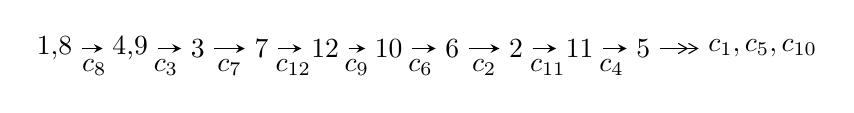
\begin{tikzpicture}[x=23pt, y=7pt]
	% node
	\node (A0) at (-1/8, 0) {1,8};
	\node (A1) at (17/16, 0) {4,9};
	\node (A2) at (17/8, 0) {3};
	\node (A3) at (25/8, 0) {7};
	\node (A4) at (33/8, 0) {12};
	\node (A5) at (41/8, 0) {10};
	\node (A6) at (49/8, 0) {6};
	\node (A7) at (57/8, 0) {2};
	\node (A8) at (65/8, 0) {11};
	\node (A9) at (73/8, 0) {5};
	\node (C1) at (1/2, -1) {$c_{8}$};
	\node (C2) at (13/8, -1) {$c_{3}$};
	\node (C3) at (21/8, -1) {$c_{7}$};
	\node (C4) at (29/8, -1) {$c_{12}$};
	\node (C5) at (37/8, -1) {$c_{9}$};
	\node (C6) at (45/8, -1) {$c_{6}$};
	\node (C7) at (53/8, -1) {$c_{2}$};
	\node (C8) at (61/8, -1) {$c_{11}$};
	\node (C9) at (69/8, -1) {$c_{4}$};
	\node (A10) at (11, 0) {$c_{1},c_{5},c_{10}$};

	% edge
	\draw[->,>=stealth]	
	(A0) edge (A1) (A1) edge (A2) (A2) edge (A3) (A3) edge (A4) (A4) edge (A5) (A5) edge (A6) (A6) edge (A7) (A7) edge (A8) (A8) edge (A9) ;
	\draw[->>,>={angle 60}]	
	(A9) edge (A10);
\end{tikzpicture} \\ 

\end{tabular} \\

\footnotetext{
The image of knot diagram is generated by the software ``\textbf{Draw programme}" developed by Andrew Bartholomew(\url{http://www.layer8.co.uk/maths/draw/index.htm\#Running-draw}), where we modified some parts for our purpose(\url{https://github.com/CATsTAILs/LinksPainter}).
}\phantom \\ \newline 
\centering \textbf{Ideals for irreducible components\footnotemark of $X_{\text{par}}$} 
 
\begin{align*}
I^u_{1}&=\langle 
5.21278\times10^{257} u^{106}+1.97423\times10^{258} u^{105}+\cdots+2.30315\times10^{258} b-7.00904\times10^{259},\\
\phantom{I^u_{1}}&\phantom{= \langle  }3.57975\times10^{259} u^{106}+1.24332\times10^{260} u^{105}+\cdots+1.68130\times10^{260} a-2.52211\times10^{261},\\
\phantom{I^u_{1}}&\phantom{= \langle  }u^{107}+4 u^{106}+\cdots-483 u-73\rangle \\
I^u_{2}&=\langle 
u^{28}-3 u^{27}+\cdots+b+1,\;u^{28}-3 u^{27}+\cdots+a-9 u,\;u^{29}-3 u^{28}+\cdots-2 u-1\rangle \\
\\
\end{align*}
\raggedright * 2 irreducible components of $\dim_{\mathbb{C}}=0$, with total 136 representations.\\
\footnotetext{All coefficients of polynomials are rational numbers. But the coefficients are sometimes approximated in decimal forms when there is not enough margin.}
\newpage
\renewcommand{\arraystretch}{1}
\centering \section*{I. $I^u_{1}= \langle 5.21\times10^{257} u^{106}+1.97\times10^{258} u^{105}+\cdots+2.30\times10^{258} b-7.01\times10^{259},\;3.58\times10^{259} u^{106}+1.24\times10^{260} u^{105}+\cdots+1.68\times10^{260} a-2.52\times10^{261},\;u^{107}+4 u^{106}+\cdots-483 u-73 \rangle$}
\flushleft \textbf{(i) Arc colorings}\\
\begin{tabular}{m{7pt} m{180pt} m{7pt} m{180pt} }
\flushright $a_{1}=$&$\begin{pmatrix}0\\u\end{pmatrix}$ \\
\flushright $a_{8}=$&$\begin{pmatrix}1\\0\end{pmatrix}$ \\
\flushright $a_{4}=$&$\begin{pmatrix}-0.212915 u^{106}-0.739501 u^{105}+\cdots+101.803 u+15.0010\\-0.226332 u^{106}-0.857184 u^{105}+\cdots+177.752 u+30.4323\end{pmatrix}$ \\
\flushright $a_{9}=$&$\begin{pmatrix}1\\u^2\end{pmatrix}$ \\
\flushright $a_{3}=$&$\begin{pmatrix}-0.439248 u^{106}-1.59668 u^{105}+\cdots+279.555 u+45.4333\\-0.226332 u^{106}-0.857184 u^{105}+\cdots+177.752 u+30.4323\end{pmatrix}$ \\
\flushright $a_{7}=$&$\begin{pmatrix}0.123007 u^{106}+0.551956 u^{105}+\cdots-157.461 u-29.3307\\-0.229569 u^{106}-0.814640 u^{105}+\cdots+117.742 u+14.6676\end{pmatrix}$ \\
\flushright $a_{12}=$&$\begin{pmatrix}u\\u^3+u\end{pmatrix}$ \\
\flushright $a_{10}=$&$\begin{pmatrix}u^2+1\\u^4+2 u^2\end{pmatrix}$ \\
\flushright $a_{6}=$&$\begin{pmatrix}0.00230451 u^{106}+0.0563939 u^{105}+\cdots-28.3080 u-6.07926\\-0.188322 u^{106}-0.672436 u^{105}+\cdots+120.647 u+18.4732\end{pmatrix}$ \\
\flushright $a_{2}=$&$\begin{pmatrix}-0.0594793 u^{106}-0.378432 u^{105}+\cdots+133.484 u+30.4867\\0.163564 u^{106}+0.562767 u^{105}+\cdots-66.1325 u-7.77903\end{pmatrix}$ \\
\flushright $a_{11}=$&$\begin{pmatrix}-0.246809 u^{106}-0.950539 u^{105}+\cdots+205.903 u+35.7170\\-0.0577528 u^{106}-0.148404 u^{105}+\cdots+9.54089 u+0.162526\end{pmatrix}$ \\
\flushright $a_{5}=$&$\begin{pmatrix}-0.263947 u^{106}-0.706517 u^{105}+\cdots+3.41770 u-12.5330\\-0.149436 u^{106}-0.565875 u^{105}+\cdots+79.2134 u+13.2693\end{pmatrix}$\\&\end{tabular}
\flushleft \textbf{(ii) Obstruction class $= -1$}\\~\\
\flushleft \textbf{(iii) Cusp Shapes $= 0.244162 u^{106}+1.15603 u^{105}+\cdots-309.404 u-76.0924$}\\~\\
\newpage\renewcommand{\arraystretch}{1}
\flushleft \textbf{(iv) u-Polynomials at the component}\newline \\
\begin{tabular}{m{50pt}|m{274pt}}
Crossings & \hspace{64pt}u-Polynomials at each crossing \\
\hline $$\begin{aligned}c_{1}\end{aligned}$$&$\begin{aligned}
&u^{107}+36 u^{106}+\cdots+13126 u+169
\end{aligned}$\\
\hline $$\begin{aligned}c_{2},c_{5}\end{aligned}$$&$\begin{aligned}
&u^{107}+4 u^{106}+\cdots+62 u+13
\end{aligned}$\\
\hline $$\begin{aligned}c_{3},c_{7}\end{aligned}$$&$\begin{aligned}
&u^{107}+u^{106}+\cdots+48147 u+6813
\end{aligned}$\\
\hline $$\begin{aligned}c_{4},c_{10}\end{aligned}$$&$\begin{aligned}
&u^{107}- u^{106}+\cdots+3 u+1
\end{aligned}$\\
\hline $$\begin{aligned}c_{6}\end{aligned}$$&$\begin{aligned}
&u^{107}+8 u^{106}+\cdots+543511 u+190727
\end{aligned}$\\
\hline $$\begin{aligned}c_{8},c_{9},c_{12}\end{aligned}$$&$\begin{aligned}
&u^{107}-4 u^{106}+\cdots-483 u+73
\end{aligned}$\\
\hline $$\begin{aligned}c_{11}\end{aligned}$$&$\begin{aligned}
&u^{107}-2 u^{106}+\cdots+11893095 u+1360881
\end{aligned}$\\
\hline
\end{tabular}\\~\\
\newpage\renewcommand{\arraystretch}{1}
\flushleft \textbf{(v) Riley Polynomials at the component}\newline \\
\begin{tabular}{m{50pt}|m{274pt}}
Crossings & \hspace{64pt}Riley Polynomials at each crossing \\
\hline $$\begin{aligned}c_{1}\end{aligned}$$&$\begin{aligned}
&y^{107}+84 y^{106}+\cdots+7091334 y-28561
\end{aligned}$\\
\hline $$\begin{aligned}c_{2},c_{5}\end{aligned}$$&$\begin{aligned}
&y^{107}-36 y^{106}+\cdots+13126 y-169
\end{aligned}$\\
\hline $$\begin{aligned}c_{3},c_{7}\end{aligned}$$&$\begin{aligned}
&y^{107}+105 y^{106}+\cdots+2042098101 y-46416969
\end{aligned}$\\
\hline $$\begin{aligned}c_{4},c_{10}\end{aligned}$$&$\begin{aligned}
&y^{107}+81 y^{106}+\cdots-149 y-1
\end{aligned}$\\
\hline $$\begin{aligned}c_{6}\end{aligned}$$&$\begin{aligned}
&y^{107}+50 y^{106}+\cdots-3420315175277 y-36376788529
\end{aligned}$\\
\hline $$\begin{aligned}c_{8},c_{9},c_{12}\end{aligned}$$&$\begin{aligned}
&y^{107}+118 y^{106}+\cdots-28197 y-5329
\end{aligned}$\\
\hline $$\begin{aligned}c_{11}\end{aligned}$$&$\begin{aligned}
&y^{107}+54 y^{106}+\cdots-41256150131529 y-1851997096161
\end{aligned}$\\
\hline
\end{tabular}\\~\\
\newpage\flushleft \textbf{(vi) Complex Volumes and Cusp Shapes}
$$\begin{array}{c|c|c}  
\text{Solutions to }I^u_{1}& \I (\text{vol} + \sqrt{-1}CS) & \text{Cusp shape}\\
 \hline 
\begin{aligned}
u &= \phantom{-}0.218610 + 0.960768 I \\
a &= \phantom{-}0.031709 - 0.835470 I \\
b &= \phantom{-}0.136668 + 0.794570 I\end{aligned}
 & \phantom{-}1.98878 - 1.86222 I & \phantom{-0.000000 } 0 \\ \hline\begin{aligned}
u &= \phantom{-}0.218610 - 0.960768 I \\
a &= \phantom{-}0.031709 + 0.835470 I \\
b &= \phantom{-}0.136668 - 0.794570 I\end{aligned}
 & \phantom{-}1.98878 + 1.86222 I & \phantom{-0.000000 } 0 \\ \hline\begin{aligned}
u &= \phantom{-}0.178070 + 0.949675 I \\
a &= \phantom{-}0.171856 + 1.326040 I \\
b &= \phantom{-}0.323476 - 0.368056 I\end{aligned}
 & -0.300806 + 0.353871 I & \phantom{-0.000000 } 0 \\ \hline\begin{aligned}
u &= \phantom{-}0.178070 - 0.949675 I \\
a &= \phantom{-}0.171856 - 1.326040 I \\
b &= \phantom{-}0.323476 + 0.368056 I\end{aligned}
 & -0.300806 - 0.353871 I & \phantom{-0.000000 } 0 \\ \hline\begin{aligned}
u &= -0.783922 + 0.745149 I \\
a &= -0.698638 - 0.803371 I \\
b &= -0.29188 + 1.42963 I\end{aligned}
 & \phantom{-}9.48816 + 6.75650 I & \phantom{-0.000000 } 0 \\ \hline\begin{aligned}
u &= -0.783922 - 0.745149 I \\
a &= -0.698638 + 0.803371 I \\
b &= -0.29188 - 1.42963 I\end{aligned}
 & \phantom{-}9.48816 - 6.75650 I & \phantom{-0.000000 } 0 \\ \hline\begin{aligned}
u &= -0.999180 + 0.440515 I \\
a &= \phantom{-}0.613313 + 0.313829 I \\
b &= -0.065695 - 1.351740 I\end{aligned}
 & \phantom{-}8.42811 - 0.88003 I & \phantom{-0.000000 } 0 \\ \hline\begin{aligned}
u &= -0.999180 - 0.440515 I \\
a &= \phantom{-}0.613313 - 0.313829 I \\
b &= -0.065695 + 1.351740 I\end{aligned}
 & \phantom{-}8.42811 + 0.88003 I & \phantom{-0.000000 } 0 \\ \hline\begin{aligned}
u &= -0.420955 + 0.792129 I \\
a &= -0.277410 - 0.472034 I \\
b &= \phantom{-}0.478629 + 1.266620 I\end{aligned}
 & \phantom{-}3.14366 - 3.02337 I & \phantom{-0.000000 } 0 \\ \hline\begin{aligned}
u &= -0.420955 - 0.792129 I \\
a &= -0.277410 + 0.472034 I \\
b &= \phantom{-}0.478629 - 1.266620 I\end{aligned}
 & \phantom{-}3.14366 + 3.02337 I & \phantom{-0.000000 } 0\\
 \hline 
 \end{array}$$\newpage$$\begin{array}{c|c|c}  
\text{Solutions to }I^u_{1}& \I (\text{vol} + \sqrt{-1}CS) & \text{Cusp shape}\\
 \hline 
\begin{aligned}
u &= -0.899486 + 0.659039 I \\
a &= \phantom{-}0.823880 + 0.629890 I \\
b &= \phantom{-}0.38198 - 1.51032 I\end{aligned}
 & \phantom{-}8.4150 + 12.8690 I & \phantom{-0.000000 } 0 \\ \hline\begin{aligned}
u &= -0.899486 - 0.659039 I \\
a &= \phantom{-}0.823880 - 0.629890 I \\
b &= \phantom{-}0.38198 + 1.51032 I\end{aligned}
 & \phantom{-}8.4150 - 12.8690 I & \phantom{-0.000000 } 0 \\ \hline\begin{aligned}
u &= \phantom{-}0.399707 + 1.055290 I \\
a &= -0.534124 + 0.874749 I \\
b &= -0.324208 - 0.576078 I\end{aligned}
 & \phantom{-}0.35578 - 5.00163 I & \phantom{-0.000000 } 0 \\ \hline\begin{aligned}
u &= \phantom{-}0.399707 - 1.055290 I \\
a &= -0.534124 - 0.874749 I \\
b &= -0.324208 + 0.576078 I\end{aligned}
 & \phantom{-}0.35578 + 5.00163 I & \phantom{-0.000000 } 0 \\ \hline\begin{aligned}
u &= -0.998726 + 0.597608 I \\
a &= -0.549600 - 0.314043 I \\
b &= \phantom{-}0.15549 + 1.46448 I\end{aligned}
 & \phantom{-}8.13008 - 6.62914 I & \phantom{-0.000000 } 0 \\ \hline\begin{aligned}
u &= -0.998726 - 0.597608 I \\
a &= -0.549600 + 0.314043 I \\
b &= \phantom{-}0.15549 - 1.46448 I\end{aligned}
 & \phantom{-}8.13008 + 6.62914 I & \phantom{-0.000000 } 0 \\ \hline\begin{aligned}
u &= \phantom{-}1.046100 + 0.646723 I \\
a &= -0.642818 + 0.564506 I \\
b &= -0.199047 - 1.344890 I\end{aligned}
 & \phantom{-}3.29521 - 6.21464 I & \phantom{-0.000000 } 0 \\ \hline\begin{aligned}
u &= \phantom{-}1.046100 - 0.646723 I \\
a &= -0.642818 - 0.564506 I \\
b &= -0.199047 + 1.344890 I\end{aligned}
 & \phantom{-}3.29521 + 6.21464 I & \phantom{-0.000000 } 0 \\ \hline\begin{aligned}
u &= \phantom{-}0.473375 + 1.139120 I \\
a &= \phantom{-}0.033224 - 0.777814 I \\
b &= -0.343973 + 0.921097 I\end{aligned}
 & \phantom{-}1.19870 - 2.22621 I & \phantom{-0.000000 } 0 \\ \hline\begin{aligned}
u &= \phantom{-}0.473375 - 1.139120 I \\
a &= \phantom{-}0.033224 + 0.777814 I \\
b &= -0.343973 - 0.921097 I\end{aligned}
 & \phantom{-}1.19870 + 2.22621 I & \phantom{-0.000000 } 0\\
 \hline 
 \end{array}$$\newpage$$\begin{array}{c|c|c}  
\text{Solutions to }I^u_{1}& \I (\text{vol} + \sqrt{-1}CS) & \text{Cusp shape}\\
 \hline 
\begin{aligned}
u &= -0.135722 + 1.236710 I \\
a &= \phantom{-}0.541906 - 0.835595 I \\
b &= -0.507847 + 0.864637 I\end{aligned}
 & \phantom{-}7.89506 + 3.99906 I & \phantom{-0.000000 } 0 \\ \hline\begin{aligned}
u &= -0.135722 - 1.236710 I \\
a &= \phantom{-}0.541906 + 0.835595 I \\
b &= -0.507847 - 0.864637 I\end{aligned}
 & \phantom{-}7.89506 - 3.99906 I & \phantom{-0.000000 } 0 \\ \hline\begin{aligned}
u &= \phantom{-}0.737344 + 0.114473 I \\
a &= -0.382379 + 0.206236 I \\
b &= -0.388809 + 0.493846 I\end{aligned}
 & -2.45708 + 0.94725 I & \phantom{-0.000000 } 0 \\ \hline\begin{aligned}
u &= \phantom{-}0.737344 - 0.114473 I \\
a &= -0.382379 - 0.206236 I \\
b &= -0.388809 - 0.493846 I\end{aligned}
 & -2.45708 - 0.94725 I & \phantom{-0.000000 } 0 \\ \hline\begin{aligned}
u &= \phantom{-}0.536312 + 0.497351 I \\
a &= -0.774722 - 0.446023 I \\
b &= -0.603705 + 0.015366 I\end{aligned}
 & -0.98968 - 3.39522 I & \phantom{-0.000000 } 0 \\ \hline\begin{aligned}
u &= \phantom{-}0.536312 - 0.497351 I \\
a &= -0.774722 + 0.446023 I \\
b &= -0.603705 - 0.015366 I\end{aligned}
 & -0.98968 + 3.39522 I & \phantom{-0.000000 } 0 \\ \hline\begin{aligned}
u &= \phantom{-}0.979345 + 0.811967 I \\
a &= \phantom{-}0.505582 - 0.602981 I \\
b &= \phantom{-}0.037448 + 1.353530 I\end{aligned}
 & \phantom{-}3.76717 - 0.64138 I & \phantom{-0.000000 } 0 \\ \hline\begin{aligned}
u &= \phantom{-}0.979345 - 0.811967 I \\
a &= \phantom{-}0.505582 + 0.602981 I \\
b &= \phantom{-}0.037448 - 1.353530 I\end{aligned}
 & \phantom{-}3.76717 + 0.64138 I & \phantom{-0.000000 } 0 \\ \hline\begin{aligned}
u &= \phantom{-}0.383425 + 0.615041 I \\
a &= \phantom{-}0.890349 - 0.220224 I \\
b &= \phantom{-}0.36445 + 1.57973 I\end{aligned}
 & \phantom{-}6.65627 + 1.23162 I & \phantom{-0.000000 } 0 \\ \hline\begin{aligned}
u &= \phantom{-}0.383425 - 0.615041 I \\
a &= \phantom{-}0.890349 + 0.220224 I \\
b &= \phantom{-}0.36445 - 1.57973 I\end{aligned}
 & \phantom{-}6.65627 - 1.23162 I & \phantom{-0.000000 } 0\\
 \hline 
 \end{array}$$\newpage$$\begin{array}{c|c|c}  
\text{Solutions to }I^u_{1}& \I (\text{vol} + \sqrt{-1}CS) & \text{Cusp shape}\\
 \hline 
\begin{aligned}
u &= -0.454638 + 0.534981 I \\
a &= \phantom{-}0.882894 - 0.100518 I \\
b &= \phantom{-}1.098940 - 0.341308 I\end{aligned}
 & \phantom{-}2.39167 + 7.72468 I & \phantom{-0.000000 } 0 \\ \hline\begin{aligned}
u &= -0.454638 - 0.534981 I \\
a &= \phantom{-}0.882894 + 0.100518 I \\
b &= \phantom{-}1.098940 + 0.341308 I\end{aligned}
 & \phantom{-}2.39167 - 7.72468 I & \phantom{-0.000000 } 0 \\ \hline\begin{aligned}
u &= \phantom{-}0.282605 + 1.286600 I \\
a &= \phantom{-}0.212333 - 0.050080 I \\
b &= -0.259293 + 0.506487 I\end{aligned}
 & \phantom{-}1.88632 - 2.72331 I & \phantom{-0.000000 } 0 \\ \hline\begin{aligned}
u &= \phantom{-}0.282605 - 1.286600 I \\
a &= \phantom{-}0.212333 + 0.050080 I \\
b &= -0.259293 - 0.506487 I\end{aligned}
 & \phantom{-}1.88632 + 2.72331 I & \phantom{-0.000000 } 0 \\ \hline\begin{aligned}
u &= -0.267787 + 0.619016 I \\
a &= -1.254590 - 0.606143 I \\
b &= -0.007919 + 1.214800 I\end{aligned}
 & \phantom{-}3.35613 - 1.33160 I & -4.65848 + 4.10187 I \\ \hline\begin{aligned}
u &= -0.267787 - 0.619016 I \\
a &= -1.254590 + 0.606143 I \\
b &= -0.007919 - 1.214800 I\end{aligned}
 & \phantom{-}3.35613 + 1.33160 I & -4.65848 - 4.10187 I \\ \hline\begin{aligned}
u &= -0.462761 + 0.433765 I \\
a &= \phantom{-}0.787952 - 1.141590 I \\
b &= -0.325099 - 0.050785 I\end{aligned}
 & \phantom{-}3.92673 + 0.31538 I & -6.76967 - 3.93949 I \\ \hline\begin{aligned}
u &= -0.462761 - 0.433765 I \\
a &= \phantom{-}0.787952 + 1.141590 I \\
b &= -0.325099 + 0.050785 I\end{aligned}
 & \phantom{-}3.92673 - 0.31538 I & -6.76967 + 3.93949 I \\ \hline\begin{aligned}
u &= -0.534765 + 0.320382 I \\
a &= \phantom{-}0.636795 + 0.790761 I \\
b &= \phantom{-}0.890340 + 0.146077 I\end{aligned}
 & -1.29323 + 1.53588 I & -13.42761 - 4.38329 I \\ \hline\begin{aligned}
u &= -0.534765 - 0.320382 I \\
a &= \phantom{-}0.636795 - 0.790761 I \\
b &= \phantom{-}0.890340 - 0.146077 I\end{aligned}
 & -1.29323 - 1.53588 I & -13.42761 + 4.38329 I\\
 \hline 
 \end{array}$$\newpage$$\begin{array}{c|c|c}  
\text{Solutions to }I^u_{1}& \I (\text{vol} + \sqrt{-1}CS) & \text{Cusp shape}\\
 \hline 
\begin{aligned}
u &= \phantom{-}0.476941 + 0.375324 I \\
a &= -2.54178 - 0.56211 I \\
b &= -0.004582 - 1.299540 I\end{aligned}
 & \phantom{-}5.88527 - 4.31483 I & -6.48516 + 8.06360 I \\ \hline\begin{aligned}
u &= \phantom{-}0.476941 - 0.375324 I \\
a &= -2.54178 + 0.56211 I \\
b &= -0.004582 + 1.299540 I\end{aligned}
 & \phantom{-}5.88527 + 4.31483 I & -6.48516 - 8.06360 I \\ \hline\begin{aligned}
u &= -0.203320 + 1.392950 I \\
a &= -0.605246 + 0.581908 I \\
b &= \phantom{-}0.899558 + 0.224964 I\end{aligned}
 & \phantom{-}4.16050 + 4.25687 I & \phantom{-0.000000 } 0 \\ \hline\begin{aligned}
u &= -0.203320 - 1.392950 I \\
a &= -0.605246 - 0.581908 I \\
b &= \phantom{-}0.899558 - 0.224964 I\end{aligned}
 & \phantom{-}4.16050 - 4.25687 I & \phantom{-0.000000 } 0 \\ \hline\begin{aligned}
u &= -0.318264 + 0.494085 I \\
a &= -1.39145 + 2.04833 I \\
b &= \phantom{-}0.245903 + 0.248452 I\end{aligned}
 & \phantom{-}2.23865 - 4.85466 I & -9.94637 + 0. I\phantom{ +0.000000I} \\ \hline\begin{aligned}
u &= -0.318264 - 0.494085 I \\
a &= -1.39145 - 2.04833 I \\
b &= \phantom{-}0.245903 - 0.248452 I\end{aligned}
 & \phantom{-}2.23865 + 4.85466 I & -9.94637 + 0. I\phantom{ +0.000000I} \\ \hline\begin{aligned}
u &= \phantom{-}0.513094 + 0.257335 I \\
a &= -1.40246 + 1.48229 I \\
b &= -0.181209 - 0.890527 I\end{aligned}
 & -1.33328 - 1.54721 I & -13.6640 + 4.4882 I \\ \hline\begin{aligned}
u &= \phantom{-}0.513094 - 0.257335 I \\
a &= -1.40246 - 1.48229 I \\
b &= -0.181209 + 0.890527 I\end{aligned}
 & -1.33328 + 1.54721 I & -13.6640 - 4.4882 I \\ \hline\begin{aligned}
u &= -0.420316 + 0.386592 I \\
a &= \phantom{-}1.83141 + 0.10916 I \\
b &= \phantom{-}0.339855 - 1.201640 I\end{aligned}
 & \phantom{-}2.56216 + 3.89824 I & -6.24282 - 0.67021 I \\ \hline\begin{aligned}
u &= -0.420316 - 0.386592 I \\
a &= \phantom{-}1.83141 - 0.10916 I \\
b &= \phantom{-}0.339855 + 1.201640 I\end{aligned}
 & \phantom{-}2.56216 - 3.89824 I & -6.24282 + 0.67021 I\\
 \hline 
 \end{array}$$\newpage$$\begin{array}{c|c|c}  
\text{Solutions to }I^u_{1}& \I (\text{vol} + \sqrt{-1}CS) & \text{Cusp shape}\\
 \hline 
\begin{aligned}
u &= -0.398457 + 0.405382 I \\
a &= -0.259591 + 0.248416 I \\
b &= -0.892262 + 0.384244 I\end{aligned}
 & \phantom{-}3.82071 + 2.68491 I & -7.21505 - 5.03363 I \\ \hline\begin{aligned}
u &= -0.398457 - 0.405382 I \\
a &= -0.259591 - 0.248416 I \\
b &= -0.892262 - 0.384244 I\end{aligned}
 & \phantom{-}3.82071 - 2.68491 I & -7.21505 + 5.03363 I \\ \hline\begin{aligned}
u &= -0.462411 + 0.313276 I \\
a &= \phantom{-}2.31541 + 1.59947 I \\
b &= \phantom{-}0.430288 - 1.125340 I\end{aligned}
 & \phantom{-}1.68920 + 6.25554 I & -12.0000 - 9.4737 I \\ \hline\begin{aligned}
u &= -0.462411 - 0.313276 I \\
a &= \phantom{-}2.31541 - 1.59947 I \\
b &= \phantom{-}0.430288 + 1.125340 I\end{aligned}
 & \phantom{-}1.68920 - 6.25554 I & -12.0000 + 9.4737 I \\ \hline\begin{aligned}
u &= \phantom{-}0.141009 + 0.537372 I \\
a &= \phantom{-}2.45726 - 2.14497 I \\
b &= -0.202138 + 1.255300 I\end{aligned}
 & \phantom{-}7.52473 + 2.42383 I & \phantom{-}1.87844 - 0.64135 I \\ \hline\begin{aligned}
u &= \phantom{-}0.141009 - 0.537372 I \\
a &= \phantom{-}2.45726 + 2.14497 I \\
b &= -0.202138 - 1.255300 I\end{aligned}
 & \phantom{-}7.52473 - 2.42383 I & \phantom{-}1.87844 + 0.64135 I \\ \hline\begin{aligned}
u &= -0.11088 + 1.46566 I \\
a &= \phantom{-}0.56373 + 2.06801 I \\
b &= -0.42043 - 1.41957 I\end{aligned}
 & \phantom{-}9.67450 - 0.61315 I & \phantom{-0.000000 } 0 \\ \hline\begin{aligned}
u &= -0.11088 - 1.46566 I \\
a &= \phantom{-}0.56373 - 2.06801 I \\
b &= -0.42043 + 1.41957 I\end{aligned}
 & \phantom{-}9.67450 + 0.61315 I & \phantom{-0.000000 } 0 \\ \hline\begin{aligned}
u &= \phantom{-}0.327146 + 0.408184 I \\
a &= -1.324250 + 0.413854 I \\
b &= -0.59487 - 1.55575 I\end{aligned}
 & \phantom{-}6.98229 - 4.18282 I & -3.31697 + 8.82974 I \\ \hline\begin{aligned}
u &= \phantom{-}0.327146 - 0.408184 I \\
a &= -1.324250 - 0.413854 I \\
b &= -0.59487 + 1.55575 I\end{aligned}
 & \phantom{-}6.98229 + 4.18282 I & -3.31697 - 8.82974 I\\
 \hline 
 \end{array}$$\newpage$$\begin{array}{c|c|c}  
\text{Solutions to }I^u_{1}& \I (\text{vol} + \sqrt{-1}CS) & \text{Cusp shape}\\
 \hline 
\begin{aligned}
u &= \phantom{-}0.12035 + 1.49065 I \\
a &= -0.27753 + 2.33161 I \\
b &= -0.041278 - 1.261910 I\end{aligned}
 & \phantom{-}4.60174 - 3.57807 I & \phantom{-0.000000 } 0 \\ \hline\begin{aligned}
u &= \phantom{-}0.12035 - 1.49065 I \\
a &= -0.27753 - 2.33161 I \\
b &= -0.041278 + 1.261910 I\end{aligned}
 & \phantom{-}4.60174 + 3.57807 I & \phantom{-0.000000 } 0 \\ \hline\begin{aligned}
u &= -0.11479 + 1.49478 I \\
a &= \phantom{-}0.47028 + 2.65788 I \\
b &= \phantom{-}0.287281 - 1.309610 I\end{aligned}
 & \phantom{-}7.77779 + 8.15655 I & \phantom{-0.000000 } 0 \\ \hline\begin{aligned}
u &= -0.11479 - 1.49478 I \\
a &= \phantom{-}0.47028 - 2.65788 I \\
b &= \phantom{-}0.287281 + 1.309610 I\end{aligned}
 & \phantom{-}7.77779 - 8.15655 I & \phantom{-0.000000 } 0 \\ \hline\begin{aligned}
u &= \phantom{-}0.12995 + 1.49543 I \\
a &= -1.54204 + 1.52645 I \\
b &= -0.216189 - 1.234570 I\end{aligned}
 & \phantom{-}12.10440 - 6.40349 I & \phantom{-0.000000 } 0 \\ \hline\begin{aligned}
u &= \phantom{-}0.12995 - 1.49543 I \\
a &= -1.54204 - 1.52645 I \\
b &= -0.216189 + 1.234570 I\end{aligned}
 & \phantom{-}12.10440 + 6.40349 I & \phantom{-0.000000 } 0 \\ \hline\begin{aligned}
u &= -0.16019 + 1.49679 I \\
a &= \phantom{-}0.574231 - 0.305715 I \\
b &= \phantom{-}0.235248 - 0.036144 I\end{aligned}
 & \phantom{-}10.23880 + 2.60950 I & \phantom{-0.000000 } 0 \\ \hline\begin{aligned}
u &= -0.16019 - 1.49679 I \\
a &= \phantom{-}0.574231 + 0.305715 I \\
b &= \phantom{-}0.235248 + 0.036144 I\end{aligned}
 & \phantom{-}10.23880 - 2.60950 I & \phantom{-0.000000 } 0 \\ \hline\begin{aligned}
u &= -0.12058 + 1.50794 I \\
a &= \phantom{-}0.58443 + 1.70466 I \\
b &= \phantom{-}0.58551 - 1.32593 I\end{aligned}
 & \phantom{-}8.92864 + 5.79082 I & \phantom{-0.000000 } 0 \\ \hline\begin{aligned}
u &= -0.12058 - 1.50794 I \\
a &= \phantom{-}0.58443 - 1.70466 I \\
b &= \phantom{-}0.58551 + 1.32593 I\end{aligned}
 & \phantom{-}8.92864 - 5.79082 I & \phantom{-0.000000 } 0\\
 \hline 
 \end{array}$$\newpage$$\begin{array}{c|c|c}  
\text{Solutions to }I^u_{1}& \I (\text{vol} + \sqrt{-1}CS) & \text{Cusp shape}\\
 \hline 
\begin{aligned}
u &= \phantom{-}0.05256 + 1.51396 I \\
a &= -0.217301 - 0.202081 I \\
b &= \phantom{-}1.037180 + 0.357448 I\end{aligned}
 & \phantom{-}5.95168 - 0.36025 I & \phantom{-0.000000 } 0 \\ \hline\begin{aligned}
u &= \phantom{-}0.05256 - 1.51396 I \\
a &= -0.217301 + 0.202081 I \\
b &= \phantom{-}1.037180 - 0.357448 I\end{aligned}
 & \phantom{-}5.95168 + 0.36025 I & \phantom{-0.000000 } 0 \\ \hline\begin{aligned}
u &= -0.07876 + 1.51449 I \\
a &= \phantom{-}0.701624 - 0.644270 I \\
b &= -1.45550 + 0.62207 I\end{aligned}
 & \phantom{-}10.25350 + 4.17019 I & \phantom{-0.000000 } 0 \\ \hline\begin{aligned}
u &= -0.07876 - 1.51449 I \\
a &= \phantom{-}0.701624 + 0.644270 I \\
b &= -1.45550 - 0.62207 I\end{aligned}
 & \phantom{-}10.25350 - 4.17019 I & \phantom{-0.000000 } 0 \\ \hline\begin{aligned}
u &= \phantom{-}0.10157 + 1.51875 I \\
a &= \phantom{-}0.04829 + 2.12071 I \\
b &= -0.93889 - 1.87708 I\end{aligned}
 & \phantom{-}13.5111 - 5.7274 I & \phantom{-0.000000 } 0 \\ \hline\begin{aligned}
u &= \phantom{-}0.10157 - 1.51875 I \\
a &= \phantom{-}0.04829 - 2.12071 I \\
b &= -0.93889 + 1.87708 I\end{aligned}
 & \phantom{-}13.5111 + 5.7274 I & \phantom{-0.000000 } 0 \\ \hline\begin{aligned}
u &= \phantom{-}0.141729 + 0.447070 I \\
a &= \phantom{-}0.389613 + 1.309160 I \\
b &= \phantom{-}0.484950 + 0.073373 I\end{aligned}
 & -0.558690 + 0.435240 I & -13.16075 + 1.11488 I \\ \hline\begin{aligned}
u &= \phantom{-}0.141729 - 0.447070 I \\
a &= \phantom{-}0.389613 - 1.309160 I \\
b &= \phantom{-}0.484950 - 0.073373 I\end{aligned}
 & -0.558690 - 0.435240 I & -13.16075 - 1.11488 I \\ \hline\begin{aligned}
u &= -0.04407 + 1.53395 I \\
a &= -0.636604 - 0.028543 I \\
b &= -0.491435 + 0.324169 I\end{aligned}
 & \phantom{-}9.16812 - 3.84604 I & \phantom{-0.000000 } 0 \\ \hline\begin{aligned}
u &= -0.04407 - 1.53395 I \\
a &= -0.636604 + 0.028543 I \\
b &= -0.491435 - 0.324169 I\end{aligned}
 & \phantom{-}9.16812 + 3.84604 I & \phantom{-0.000000 } 0\\
 \hline 
 \end{array}$$\newpage$$\begin{array}{c|c|c}  
\text{Solutions to }I^u_{1}& \I (\text{vol} + \sqrt{-1}CS) & \text{Cusp shape}\\
 \hline 
\begin{aligned}
u &= \phantom{-}0.02073 + 1.54207 I \\
a &= \phantom{-}0.84675 - 2.52362 I \\
b &= \phantom{-}0.017497 + 1.330960 I\end{aligned}
 & \phantom{-}14.5710 + 1.9650 I & \phantom{-0.000000 } 0 \\ \hline\begin{aligned}
u &= \phantom{-}0.02073 - 1.54207 I \\
a &= \phantom{-}0.84675 + 2.52362 I \\
b &= \phantom{-}0.017497 - 1.330960 I\end{aligned}
 & \phantom{-}14.5710 - 1.9650 I & \phantom{-0.000000 } 0 \\ \hline\begin{aligned}
u &= \phantom{-}0.16163 + 1.53836 I \\
a &= \phantom{-}0.225279 + 0.170191 I \\
b &= -1.075420 - 0.085848 I\end{aligned}
 & \phantom{-}5.83460 - 5.91752 I & \phantom{-0.000000 } 0 \\ \hline\begin{aligned}
u &= \phantom{-}0.16163 - 1.53836 I \\
a &= \phantom{-}0.225279 - 0.170191 I \\
b &= -1.075420 + 0.085848 I\end{aligned}
 & \phantom{-}5.83460 + 5.91752 I & \phantom{-0.000000 } 0 \\ \hline\begin{aligned}
u &= -0.13844 + 1.55199 I \\
a &= -0.704780 + 0.620989 I \\
b &= \phantom{-}1.65352 - 0.40742 I\end{aligned}
 & \phantom{-}9.43130 + 9.88978 I & \phantom{-0.000000 } 0 \\ \hline\begin{aligned}
u &= -0.13844 - 1.55199 I \\
a &= -0.704780 - 0.620989 I \\
b &= \phantom{-}1.65352 + 0.40742 I\end{aligned}
 & \phantom{-}9.43130 - 9.88978 I & \phantom{-0.000000 } 0 \\ \hline\begin{aligned}
u &= -0.03795 + 1.56754 I \\
a &= -0.30023 - 1.90446 I \\
b &= -0.29998 + 1.49901 I\end{aligned}
 & \phantom{-}10.81920 - 0.43166 I & \phantom{-0.000000 } 0 \\ \hline\begin{aligned}
u &= -0.03795 - 1.56754 I \\
a &= -0.30023 + 1.90446 I \\
b &= -0.29998 - 1.49901 I\end{aligned}
 & \phantom{-}10.81920 + 0.43166 I & \phantom{-0.000000 } 0 \\ \hline\begin{aligned}
u &= \phantom{-}0.07869 + 1.58239 I \\
a &= -0.06364 - 1.99815 I \\
b &= \phantom{-}0.74333 + 2.06303 I\end{aligned}
 & \phantom{-}14.1741 - 0.3259 I & \phantom{-0.000000 } 0 \\ \hline\begin{aligned}
u &= \phantom{-}0.07869 - 1.58239 I \\
a &= -0.06364 + 1.99815 I \\
b &= \phantom{-}0.74333 - 2.06303 I\end{aligned}
 & \phantom{-}14.1741 + 0.3259 I & \phantom{-0.000000 } 0\\
 \hline 
 \end{array}$$\newpage$$\begin{array}{c|c|c}  
\text{Solutions to }I^u_{1}& \I (\text{vol} + \sqrt{-1}CS) & \text{Cusp shape}\\
 \hline 
\begin{aligned}
u &= -0.23936 + 1.61844 I \\
a &= -0.48005 - 1.89887 I \\
b &= -0.43878 + 1.61218 I\end{aligned}
 & \phantom{-}17.3391 + 10.5622 I & \phantom{-0.000000 } 0 \\ \hline\begin{aligned}
u &= -0.23936 - 1.61844 I \\
a &= -0.48005 + 1.89887 I \\
b &= -0.43878 - 1.61218 I\end{aligned}
 & \phantom{-}17.3391 - 10.5622 I & \phantom{-0.000000 } 0 \\ \hline\begin{aligned}
u &= -0.30020 + 1.60868 I \\
a &= \phantom{-}0.61408 + 1.79515 I \\
b &= \phantom{-}0.55307 - 1.62905 I\end{aligned}
 & \phantom{-}15.8563 + 17.3211 I & \phantom{-0.000000 } 0 \\ \hline\begin{aligned}
u &= -0.30020 - 1.60868 I \\
a &= \phantom{-}0.61408 - 1.79515 I \\
b &= \phantom{-}0.55307 + 1.62905 I\end{aligned}
 & \phantom{-}15.8563 - 17.3211 I & \phantom{-0.000000 } 0 \\ \hline\begin{aligned}
u &= -0.39503 + 1.59788 I \\
a &= \phantom{-}0.76123 + 1.40447 I \\
b &= \phantom{-}0.166532 - 1.386090 I\end{aligned}
 & \phantom{-}15.0145 + 4.3541 I & \phantom{-0.000000 } 0 \\ \hline\begin{aligned}
u &= -0.39503 - 1.59788 I \\
a &= \phantom{-}0.76123 - 1.40447 I \\
b &= \phantom{-}0.166532 + 1.386090 I\end{aligned}
 & \phantom{-}15.0145 - 4.3541 I & \phantom{-0.000000 } 0 \\ \hline\begin{aligned}
u &= -0.05430 + 1.65387 I \\
a &= -0.22797 - 1.75899 I \\
b &= \phantom{-}0.15024 + 1.86593 I\end{aligned}
 & \phantom{-}11.86160 - 1.46045 I & \phantom{-0.000000 } 0 \\ \hline\begin{aligned}
u &= -0.05430 - 1.65387 I \\
a &= -0.22797 + 1.75899 I \\
b &= \phantom{-}0.15024 - 1.86593 I\end{aligned}
 & \phantom{-}11.86160 + 1.46045 I & \phantom{-0.000000 } 0 \\ \hline\begin{aligned}
u &= -0.325540 + 0.093169 I \\
a &= \phantom{-}1.53708 + 0.78756 I \\
b &= -0.548176 - 0.981523 I\end{aligned}
 & \phantom{-}4.26238 - 2.15362 I & -14.5846 + 5.0933 I \\ \hline\begin{aligned}
u &= -0.325540 - 0.093169 I \\
a &= \phantom{-}1.53708 - 0.78756 I \\
b &= -0.548176 + 0.981523 I\end{aligned}
 & \phantom{-}4.26238 + 2.15362 I & -14.5846 - 5.0933 I\\
 \hline 
 \end{array}$$\newpage$$\begin{array}{c|c|c}  
\text{Solutions to }I^u_{1}& \I (\text{vol} + \sqrt{-1}CS) & \text{Cusp shape}\\
 \hline 
\begin{aligned}
u &= \phantom{-}0.32722 + 1.63615 I \\
a &= -0.59621 + 1.60182 I \\
b &= -0.43198 - 1.44422 I\end{aligned}
 & \phantom{-}10.8326 - 11.2575 I & \phantom{-0.000000 } 0 \\ \hline\begin{aligned}
u &= \phantom{-}0.32722 - 1.63615 I \\
a &= -0.59621 - 1.60182 I \\
b &= -0.43198 + 1.44422 I\end{aligned}
 & \phantom{-}10.8326 + 11.2575 I & \phantom{-0.000000 } 0 \\ \hline\begin{aligned}
u &= \phantom{-}0.24302 + 1.66340 I \\
a &= \phantom{-}0.41953 - 1.67154 I \\
b &= \phantom{-}0.31142 + 1.51218 I\end{aligned}
 & \phantom{-}12.18450 - 5.07799 I & \phantom{-0.000000 } 0 \\ \hline\begin{aligned}
u &= \phantom{-}0.24302 - 1.66340 I \\
a &= \phantom{-}0.41953 + 1.67154 I \\
b &= \phantom{-}0.31142 - 1.51218 I\end{aligned}
 & \phantom{-}12.18450 + 5.07799 I & \phantom{-0.000000 } 0 \\ \hline\begin{aligned}
u &= -0.32773 + 1.67521 I \\
a &= -0.59722 - 1.42967 I \\
b &= -0.12777 + 1.53523 I\end{aligned}
 & \phantom{-}15.6605 - 1.5214 I & \phantom{-0.000000 } 0 \\ \hline\begin{aligned}
u &= -0.32773 - 1.67521 I \\
a &= -0.59722 + 1.42967 I \\
b &= -0.12777 - 1.53523 I\end{aligned}
 & \phantom{-}15.6605 + 1.5214 I & \phantom{-0.000000 } 0 \\ \hline\begin{aligned}
u &= \phantom{-}0.275965\phantom{ +0.000000I} \\
a &= -0.570569\phantom{ +0.000000I} \\
b &= \phantom{-}0.339181\phantom{ +0.000000I}\end{aligned}
 & -0.579142\phantom{ +0.000000I} & -17.1090\phantom{ +0.000000I}\\
 \hline 
 \end{array}$$\newpage\newpage\renewcommand{\arraystretch}{1}
\centering \section*{II. $I^u_{2}= \langle u^{28}-3 u^{27}+\cdots+b+1,\;u^{28}-3 u^{27}+\cdots+a-9 u,\;u^{29}-3 u^{28}+\cdots-2 u-1 \rangle$}
\flushleft \textbf{(i) Arc colorings}\\
\begin{tabular}{m{7pt} m{180pt} m{7pt} m{180pt} }
\flushright $a_{1}=$&$\begin{pmatrix}0\\u\end{pmatrix}$ \\
\flushright $a_{8}=$&$\begin{pmatrix}1\\0\end{pmatrix}$ \\
\flushright $a_{4}=$&$\begin{pmatrix}- u^{28}+3 u^{27}+\cdots+9 u^2+9 u\\- u^{28}+3 u^{27}+\cdots- u-1\end{pmatrix}$ \\
\flushright $a_{9}=$&$\begin{pmatrix}1\\u^2\end{pmatrix}$ \\
\flushright $a_{3}=$&$\begin{pmatrix}-2 u^{28}+6 u^{27}+\cdots+8 u-1\\- u^{28}+3 u^{27}+\cdots- u-1\end{pmatrix}$ \\
\flushright $a_{7}=$&$\begin{pmatrix}- u^{26}+4 u^{25}+\cdots-2 u-1\\- u^5+u^4-3 u^3+2 u^2-2 u+1\end{pmatrix}$ \\
\flushright $a_{12}=$&$\begin{pmatrix}u\\u^3+u\end{pmatrix}$ \\
\flushright $a_{10}=$&$\begin{pmatrix}u^2+1\\u^4+2 u^2\end{pmatrix}$ \\
\flushright $a_{6}=$&$\begin{pmatrix}- u^{26}+4 u^{25}+\cdots-4 u-1\\- u^{28}+3 u^{27}+\cdots- u+1\end{pmatrix}$ \\
\flushright $a_{2}=$&$\begin{pmatrix}- u^{28}+3 u^{27}+\cdots-3 u-6\\- u^{27}+4 u^{26}+\cdots+11 u^3-4 u^2\end{pmatrix}$ \\
\flushright $a_{11}=$&$\begin{pmatrix}- u^{26}+3 u^{25}+\cdots+6 u^2+9 u\\u^{28}-3 u^{27}+\cdots-2 u-2\end{pmatrix}$ \\
\flushright $a_{5}=$&$\begin{pmatrix}- u^{28}+3 u^{27}+\cdots+5 u+4\\u^{27}-4 u^{26}+\cdots-2 u-1\end{pmatrix}$\\&\end{tabular}
\flushleft \textbf{(ii) Obstruction class $= 1$}\\~\\
\flushleft \textbf{(iii) Cusp Shapes $= -2 u^{28}+2 u^{27}-35 u^{26}+40 u^{25}-287 u^{24}+347 u^{23}-1444 u^{22}+1720 u^{21}-4869 u^{20}+5365 u^{19}-11288 u^{18}+10857 u^{17}-17856 u^{16}+14038 u^{15}-18593 u^{14}+10722 u^{13}-11806 u^{12}+3674 u^{11}-3899 u^{10}-380 u^9-483 u^8-446 u^7-52 u^6+66 u^5+31 u^4+77 u^3+39 u^2+27 u+2$}\\~\\
\newpage\renewcommand{\arraystretch}{1}
\flushleft \textbf{(iv) u-Polynomials at the component}\newline \\
\begin{tabular}{m{50pt}|m{274pt}}
Crossings & \hspace{64pt}u-Polynomials at each crossing \\
\hline $$\begin{aligned}c_{1}\end{aligned}$$&$\begin{aligned}
&u^{29}-13 u^{28}+\cdots+13 u-1
\end{aligned}$\\
\hline $$\begin{aligned}c_{2}\end{aligned}$$&$\begin{aligned}
&u^{29}+3 u^{28}+\cdots-3 u-1
\end{aligned}$\\
\hline $$\begin{aligned}c_{3}\end{aligned}$$&$\begin{aligned}
&u^{29}+16 u^{27}+\cdots+8 u-1
\end{aligned}$\\
\hline $$\begin{aligned}c_{4}\end{aligned}$$&$\begin{aligned}
&u^{29}+10 u^{27}+\cdots-2 u+1
\end{aligned}$\\
\hline $$\begin{aligned}c_{5}\end{aligned}$$&$\begin{aligned}
&u^{29}-3 u^{28}+\cdots-3 u+1
\end{aligned}$\\
\hline $$\begin{aligned}c_{6}\end{aligned}$$&$\begin{aligned}
&u^{29}- u^{28}+\cdots-7 u^2-1
\end{aligned}$\\
\hline $$\begin{aligned}c_{7}\end{aligned}$$&$\begin{aligned}
&u^{29}+16 u^{27}+\cdots+8 u+1
\end{aligned}$\\
\hline $$\begin{aligned}c_{8},c_{9}\end{aligned}$$&$\begin{aligned}
&u^{29}-3 u^{28}+\cdots-2 u-1
\end{aligned}$\\
\hline $$\begin{aligned}c_{10}\end{aligned}$$&$\begin{aligned}
&u^{29}+10 u^{27}+\cdots-2 u-1
\end{aligned}$\\
\hline $$\begin{aligned}c_{11}\end{aligned}$$&$\begin{aligned}
&u^{29}+u^{28}+\cdots+13 u^2+1
\end{aligned}$\\
\hline $$\begin{aligned}c_{12}\end{aligned}$$&$\begin{aligned}
&u^{29}+3 u^{28}+\cdots-2 u+1
\end{aligned}$\\
\hline
\end{tabular}\\~\\
\newpage\renewcommand{\arraystretch}{1}
\flushleft \textbf{(v) Riley Polynomials at the component}\newline \\
\begin{tabular}{m{50pt}|m{274pt}}
Crossings & \hspace{64pt}Riley Polynomials at each crossing \\
\hline $$\begin{aligned}c_{1}\end{aligned}$$&$\begin{aligned}
&y^{29}+19 y^{28}+\cdots-11 y-1
\end{aligned}$\\
\hline $$\begin{aligned}c_{2},c_{5}\end{aligned}$$&$\begin{aligned}
&y^{29}-13 y^{28}+\cdots+13 y-1
\end{aligned}$\\
\hline $$\begin{aligned}c_{3},c_{7}\end{aligned}$$&$\begin{aligned}
&y^{29}+32 y^{28}+\cdots-16 y-1
\end{aligned}$\\
\hline $$\begin{aligned}c_{4},c_{10}\end{aligned}$$&$\begin{aligned}
&y^{29}+20 y^{28}+\cdots+26 y-1
\end{aligned}$\\
\hline $$\begin{aligned}c_{6}\end{aligned}$$&$\begin{aligned}
&y^{29}+9 y^{28}+\cdots-14 y-1
\end{aligned}$\\
\hline $$\begin{aligned}c_{8},c_{9},c_{12}\end{aligned}$$&$\begin{aligned}
&y^{29}+33 y^{28}+\cdots-10 y-1
\end{aligned}$\\
\hline $$\begin{aligned}c_{11}\end{aligned}$$&$\begin{aligned}
&y^{29}+9 y^{28}+\cdots-26 y-1
\end{aligned}$\\
\hline
\end{tabular}\\~\\
\newpage\flushleft \textbf{(vi) Complex Volumes and Cusp Shapes}
$$\begin{array}{c|c|c}  
\text{Solutions to }I^u_{2}& \I (\text{vol} + \sqrt{-1}CS) & \text{Cusp shape}\\
 \hline 
\begin{aligned}
u &= \phantom{-}0.320010 + 0.929198 I \\
a &= \phantom{-}0.39466 + 1.70289 I \\
b &= \phantom{-}0.038419 - 0.734900 I\end{aligned}
 & \phantom{-}0.433243 + 0.124395 I & -4.84474 + 0.20044 I \\ \hline\begin{aligned}
u &= \phantom{-}0.320010 - 0.929198 I \\
a &= \phantom{-}0.39466 - 1.70289 I \\
b &= \phantom{-}0.038419 + 0.734900 I\end{aligned}
 & \phantom{-}0.433243 - 0.124395 I & -4.84474 - 0.20044 I \\ \hline\begin{aligned}
u &= \phantom{-}0.619532 + 0.742782 I \\
a &= -1.056600 + 0.712156 I \\
b &= -0.215695 - 1.137310 I\end{aligned}
 & \phantom{-}2.22927 - 4.93398 I & -8.38230 + 6.45291 I \\ \hline\begin{aligned}
u &= \phantom{-}0.619532 - 0.742782 I \\
a &= -1.056600 - 0.712156 I \\
b &= -0.215695 + 1.137310 I\end{aligned}
 & \phantom{-}2.22927 + 4.93398 I & -8.38230 - 6.45291 I \\ \hline\begin{aligned}
u &= \phantom{-}0.643736 + 0.904472 I \\
a &= \phantom{-}0.683690 - 0.546558 I \\
b &= -0.044141 + 1.253420 I\end{aligned}
 & \phantom{-}2.67368 + 0.08755 I & -9.01016 - 0.85925 I \\ \hline\begin{aligned}
u &= \phantom{-}0.643736 - 0.904472 I \\
a &= \phantom{-}0.683690 + 0.546558 I \\
b &= -0.044141 - 1.253420 I\end{aligned}
 & \phantom{-}2.67368 - 0.08755 I & -9.01016 + 0.85925 I \\ \hline\begin{aligned}
u &= \phantom{-}0.409561 + 1.069620 I \\
a &= -0.284586 - 0.522394 I \\
b &= -0.295871 + 0.778735 I\end{aligned}
 & \phantom{-}1.02762 - 2.88773 I & -9.85449 + 8.09995 I \\ \hline\begin{aligned}
u &= \phantom{-}0.409561 - 1.069620 I \\
a &= -0.284586 + 0.522394 I \\
b &= -0.295871 - 0.778735 I\end{aligned}
 & \phantom{-}1.02762 + 2.88773 I & -9.85449 - 8.09995 I \\ \hline\begin{aligned}
u &= -0.142765 + 1.249060 I \\
a &= -0.833830 + 1.067700 I \\
b &= \phantom{-}0.601906 - 0.712923 I\end{aligned}
 & \phantom{-}7.51370 + 3.35651 I & -8.50874 + 0.95421 I \\ \hline\begin{aligned}
u &= -0.142765 - 1.249060 I \\
a &= -0.833830 - 1.067700 I \\
b &= \phantom{-}0.601906 + 0.712923 I\end{aligned}
 & \phantom{-}7.51370 - 3.35651 I & -8.50874 - 0.95421 I\\
 \hline 
 \end{array}$$\newpage$$\begin{array}{c|c|c}  
\text{Solutions to }I^u_{2}& \I (\text{vol} + \sqrt{-1}CS) & \text{Cusp shape}\\
 \hline 
\begin{aligned}
u &= -0.062902 + 1.256950 I \\
a &= \phantom{-}1.177200 + 0.201358 I \\
b &= -0.382326 + 0.682765 I\end{aligned}
 & \phantom{-}5.57353 + 6.14807 I & -6.11924 - 5.75813 I \\ \hline\begin{aligned}
u &= -0.062902 - 1.256950 I \\
a &= \phantom{-}1.177200 - 0.201358 I \\
b &= -0.382326 - 0.682765 I\end{aligned}
 & \phantom{-}5.57353 - 6.14807 I & -6.11924 + 5.75813 I \\ \hline\begin{aligned}
u &= \phantom{-}0.219923 + 1.280020 I \\
a &= -0.089089 + 0.378279 I \\
b &= -0.162580 + 0.225216 I\end{aligned}
 & \phantom{-}1.55717 - 3.04406 I & -15.4554 + 7.1702 I \\ \hline\begin{aligned}
u &= \phantom{-}0.219923 - 1.280020 I \\
a &= -0.089089 - 0.378279 I \\
b &= -0.162580 - 0.225216 I\end{aligned}
 & \phantom{-}1.55717 + 3.04406 I & -15.4554 - 7.1702 I \\ \hline\begin{aligned}
u &= \phantom{-}0.615147\phantom{ +0.000000I} \\
a &= -0.815486\phantom{ +0.000000I} \\
b &= -0.341615\phantom{ +0.000000I}\end{aligned}
 & -2.42903\phantom{ +0.000000I} & -16.1420\phantom{ +0.000000I} \\ \hline\begin{aligned}
u &= -0.15234 + 1.44097 I \\
a &= \phantom{-}0.77709 + 1.42350 I \\
b &= \phantom{-}0.446284 - 1.339670 I\end{aligned}
 & \phantom{-}11.44890 + 5.04952 I & -4.21898 - 2.62364 I \\ \hline\begin{aligned}
u &= -0.15234 - 1.44097 I \\
a &= \phantom{-}0.77709 - 1.42350 I \\
b &= \phantom{-}0.446284 + 1.339670 I\end{aligned}
 & \phantom{-}11.44890 - 5.04952 I & -4.21898 + 2.62364 I \\ \hline\begin{aligned}
u &= -0.263492 + 0.446508 I \\
a &= \phantom{-}0.390765 - 1.123370 I \\
b &= \phantom{-}0.590532 + 1.084710 I\end{aligned}
 & \phantom{-}4.70619 - 1.81374 I & -2.21768 - 3.11805 I \\ \hline\begin{aligned}
u &= -0.263492 - 0.446508 I \\
a &= \phantom{-}0.390765 + 1.123370 I \\
b &= \phantom{-}0.590532 - 1.084710 I\end{aligned}
 & \phantom{-}4.70619 + 1.81374 I & -2.21768 + 3.11805 I \\ \hline\begin{aligned}
u &= -0.019923 + 0.460345 I \\
a &= -2.10006 + 3.07543 I \\
b &= -0.385295 - 0.880991 I\end{aligned}
 & \phantom{-}2.73526 - 5.65484 I & -4.63168 + 7.14796 I\\
 \hline 
 \end{array}$$\newpage$$\begin{array}{c|c|c}  
\text{Solutions to }I^u_{2}& \I (\text{vol} + \sqrt{-1}CS) & \text{Cusp shape}\\
 \hline 
\begin{aligned}
u &= -0.019923 - 0.460345 I \\
a &= -2.10006 - 3.07543 I \\
b &= -0.385295 + 0.880991 I\end{aligned}
 & \phantom{-}2.73526 + 5.65484 I & -4.63168 - 7.14796 I \\ \hline\begin{aligned}
u &= \phantom{-}0.09517 + 1.53920 I \\
a &= -0.61440 + 1.61562 I \\
b &= -0.599071 - 1.143990 I\end{aligned}
 & \phantom{-}9.89424 - 6.58410 I & -3.77263 + 5.83456 I \\ \hline\begin{aligned}
u &= \phantom{-}0.09517 - 1.53920 I \\
a &= -0.61440 - 1.61562 I \\
b &= -0.599071 + 1.143990 I\end{aligned}
 & \phantom{-}9.89424 + 6.58410 I & -3.77263 - 5.83456 I \\ \hline\begin{aligned}
u &= -0.09903 + 1.55874 I \\
a &= -0.50230 - 1.90709 I \\
b &= -0.04502 + 1.69043 I\end{aligned}
 & \phantom{-}12.87670 - 1.34074 I & -2.57674 + 2.90001 I \\ \hline\begin{aligned}
u &= -0.09903 - 1.55874 I \\
a &= -0.50230 + 1.90709 I \\
b &= -0.04502 - 1.69043 I\end{aligned}
 & \phantom{-}12.87670 + 1.34074 I & -2.57674 - 2.90001 I \\ \hline\begin{aligned}
u &= -0.01439 + 1.61720 I \\
a &= -0.13191 - 1.82061 I \\
b &= \phantom{-}0.42135 + 1.72225 I\end{aligned}
 & \phantom{-}12.44350 - 0.92978 I & -2.68721 + 0. I\phantom{ +0.000000I} \\ \hline\begin{aligned}
u &= -0.01439 - 1.61720 I \\
a &= -0.13191 + 1.82061 I \\
b &= \phantom{-}0.42135 - 1.72225 I\end{aligned}
 & \phantom{-}12.44350 + 0.92978 I & -2.68721 + 0. I\phantom{ +0.000000I} \\ \hline\begin{aligned}
u &= -0.360674 + 0.121864 I \\
a &= -1.40289 + 1.84758 I \\
b &= \phantom{-}0.20232 + 1.44582 I\end{aligned}
 & \phantom{-}6.70328 - 3.10811 I & -5.14888 + 2.92110 I \\ \hline\begin{aligned}
u &= -0.360674 - 0.121864 I \\
a &= -1.40289 - 1.84758 I \\
b &= \phantom{-}0.20232 - 1.44582 I\end{aligned}
 & \phantom{-}6.70328 + 3.10811 I & -5.14888 - 2.92110 I\\
 \hline 
 \end{array}$$\newpage
\newpage\renewcommand{\arraystretch}{1}
\centering \section*{ III. u-Polynomials}
\begin{tabular}{m{50pt}|m{274pt}}
Crossings & \hspace{64pt}u-Polynomials at each crossing \\
\hline $$\begin{aligned}c_{1}\end{aligned}$$&$\begin{aligned}
&(u^{29}-13 u^{28}+\cdots+13 u-1)(u^{107}+36 u^{106}+\cdots+13126 u+169)
\end{aligned}$\\
\hline $$\begin{aligned}c_{2}\end{aligned}$$&$\begin{aligned}
&(u^{29}+3 u^{28}+\cdots-3 u-1)(u^{107}+4 u^{106}+\cdots+62 u+13)
\end{aligned}$\\
\hline $$\begin{aligned}c_{3}\end{aligned}$$&$\begin{aligned}
&(u^{29}+16 u^{27}+\cdots+8 u-1)(u^{107}+u^{106}+\cdots+48147 u+6813)
\end{aligned}$\\
\hline $$\begin{aligned}c_{4}\end{aligned}$$&$\begin{aligned}
&(u^{29}+10 u^{27}+\cdots-2 u+1)(u^{107}- u^{106}+\cdots+3 u+1)
\end{aligned}$\\
\hline $$\begin{aligned}c_{5}\end{aligned}$$&$\begin{aligned}
&(u^{29}-3 u^{28}+\cdots-3 u+1)(u^{107}+4 u^{106}+\cdots+62 u+13)
\end{aligned}$\\
\hline $$\begin{aligned}c_{6}\end{aligned}$$&$\begin{aligned}
&(u^{29}- u^{28}+\cdots-7 u^2-1)(u^{107}+8 u^{106}+\cdots+543511 u+190727)
\end{aligned}$\\
\hline $$\begin{aligned}c_{7}\end{aligned}$$&$\begin{aligned}
&(u^{29}+16 u^{27}+\cdots+8 u+1)(u^{107}+u^{106}+\cdots+48147 u+6813)
\end{aligned}$\\
\hline $$\begin{aligned}c_{8},c_{9}\end{aligned}$$&$\begin{aligned}
&(u^{29}-3 u^{28}+\cdots-2 u-1)(u^{107}-4 u^{106}+\cdots-483 u+73)
\end{aligned}$\\
\hline $$\begin{aligned}c_{10}\end{aligned}$$&$\begin{aligned}
&(u^{29}+10 u^{27}+\cdots-2 u-1)(u^{107}- u^{106}+\cdots+3 u+1)
\end{aligned}$\\
\hline $$\begin{aligned}c_{11}\end{aligned}$$&$\begin{aligned}
&(u^{29}+u^{28}+\cdots+13 u^2+1)\\
&\cdot(u^{107}-2 u^{106}+\cdots+11893095 u+1360881)
\end{aligned}$\\
\hline $$\begin{aligned}c_{12}\end{aligned}$$&$\begin{aligned}
&(u^{29}+3 u^{28}+\cdots-2 u+1)(u^{107}-4 u^{106}+\cdots-483 u+73)
\end{aligned}$\\
\hline
\end{tabular}\newpage\renewcommand{\arraystretch}{1}
\centering \section*{ IV. Riley Polynomials}
\begin{tabular}{m{50pt}|m{274pt}}
Crossings & \hspace{64pt}Riley Polynomials at each crossing \\
\hline $$\begin{aligned}c_{1}\end{aligned}$$&$\begin{aligned}
&(y^{29}+19 y^{28}+\cdots-11 y-1)\\
&\cdot(y^{107}+84 y^{106}+\cdots+7091334 y-28561)
\end{aligned}$\\
\hline $$\begin{aligned}c_{2},c_{5}\end{aligned}$$&$\begin{aligned}
&(y^{29}-13 y^{28}+\cdots+13 y-1)(y^{107}-36 y^{106}+\cdots+13126 y-169)
\end{aligned}$\\
\hline $$\begin{aligned}c_{3},c_{7}\end{aligned}$$&$\begin{aligned}
&(y^{29}+32 y^{28}+\cdots-16 y-1)\\
&\cdot(y^{107}+105 y^{106}+\cdots+2042098101 y-46416969)
\end{aligned}$\\
\hline $$\begin{aligned}c_{4},c_{10}\end{aligned}$$&$\begin{aligned}
&(y^{29}+20 y^{28}+\cdots+26 y-1)(y^{107}+81 y^{106}+\cdots-149 y-1)
\end{aligned}$\\
\hline $$\begin{aligned}c_{6}\end{aligned}$$&$\begin{aligned}
&(y^{29}+9 y^{28}+\cdots-14 y-1)\\
&\cdot(y^{107}+50 y^{106}+\cdots-3420315175277 y-36376788529)
\end{aligned}$\\
\hline $$\begin{aligned}c_{8},c_{9},c_{12}\end{aligned}$$&$\begin{aligned}
&(y^{29}+33 y^{28}+\cdots-10 y-1)(y^{107}+118 y^{106}+\cdots-28197 y-5329)
\end{aligned}$\\
\hline $$\begin{aligned}c_{11}\end{aligned}$$&$\begin{aligned}
&(y^{29}+9 y^{28}+\cdots-26 y-1)\\
&\cdot(y^{107}+54 y^{106}+\cdots-41256150131529 y-1851997096161)
\end{aligned}$\\
\hline
\end{tabular}
\vskip 2pc
\end{document}